% Chapter 2

\chapter{Protocolo HTTP} % Chapter title

\label{ch:protocolo_http} % For referencing the chapter elsewhere, use \autoref{ch:protocolo_http} 

%----------------------------------------------------------------------------------------

\lipsum[1]

%----------------------------------------------------------------------------------------

\section{¿Cómo trabaja?}

El protocolo HTTP es un protocolo petición/respuesta. Un cliente envía una petición al servidor en la forma de un método de petición, URI, versión de protocolo, seguido de un mensaje estilo-
MIME conteniendo los modificadores de la petición, información del cliente y posiblemente el contenido del cuerpo sobre una conexión con el servidor, el servidor resuelve con un mensaje de estatus, incluyendo la versión del protocolo del mensaje y el código de error o éxito, seguido de un mensaje estilo-MIME que contiene la información del servidor, la meta-información de la entidad y posiblemente el contenido del cuerpo de la entidad.
La conexión más simple seria en la cual el agente de usuario realice una conexión directa con el servidor de origen, entonces la conexión de una petición seria:

\begin{figure}[h]
  \centering
    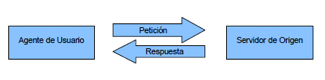
\includegraphics[scale=1]{gfx/conexion_http}
  \caption{Conexión HTTP}
  \label{conexionhttp}
\end{figure}


En conexiones más complejas pueden intervenir uno o más intermediarios, como lo pueden ser:

  \begin{itemize}
     \item Proxies que son agentes de reenvío, este recibe peticiones para un URI en su forma absoluta, sobre escribe toda o parte del mensaje y reenvía las peticiones re-formateadas hacia el servidor identificado por la URI.
     \item Gateway es un agente de recepción, actuando como una capa sobre otros servidores y si es necesario traduce la petición al protocolo del servidor subyacente.
     \item Túnel: Actúa como un punto de transmisión entre dos conexiones sin cambiar el mensaje, los túneles son usados cuando la conexión pasa a través de un intermediario (como un firewall) aun cuando el intermediario no entiende los contenidos del mensaje.
  \end{itemize}


%------------------------------------------------
\section{Mensajes HTTP}

\begin{description}
\item[Tipos de Mensajes:] 

Los tipos de mensajes HTTP son de petición de un cliente hacia el servidor y de respuesta de un servidor hacia el cliente.

\begin{verbatim}
“HTTP-message = Request | Response ; HTTP/1.1 messages”
\end{verbatim}

Los mensajes utilizan la forma genérica de mensajes, definido en RFC822 para transferencia de mensajes. Ambos mensajes consisten una línea de inicio, uno o más valores de encabezado, una línea vacía que indica el final de los valores de encabezado y posiblemente un cuerpo del mensaje.

\item[Encabezados del Mensaje:] 
Los valores HTTP, los cuales incluyen general-header, request-header, response-header y entityheader, siguen el mismo formato genérico del RFC822. Cada campo del encabezado consiste de un nombre seguido por “:” y un valor. Los nombres de campos son case-insensitive y el valor se puede extender múltiples líneas.
\item[Cuerpo del Mensaje:] 

El cuerpo del mensaje de un mensaje HTTP es utilizado para trasportar el cuerpo de la entidad asociado con la respuesta o la petición. El cuerpo del mensaje difiere del cuerpo de la entidad solo cuando una codificación de transferencia ha sido aplicada. “message-body = entity-body | entity-body codificado”  
El campo Transfer-Encoding debe ser utilizado para indicar cualquier codificación de transferencia aplicada por una aplicación para asegurar la transferencia adecuada del mensaje. Transfer-Encoding es una propiedad del mensaje no de la entidad.

\item[Largo del Mensaje:] 

El transfer-length de un mensaje es el largo del cuerpo del mensaje a como este aparece en el mensaje, que es, sin que se le allá aplicado ningún filtro. Cuando el cuerpo del mensaje es incluido con un mensaje, el transfer-length de ese cuerpo es determinado por uno de:
\begin{itemize}

\item Cualquier mensaje de respuesta que no incluya cuerpo del mensaje como las repuestas estatus 204 y 304 son siempre terminadas con la primer línea vacía después de los campos de encabezado presentes en el mensaje.
\item Si un campo de Transfer-Encoding se encuentra especificado y tiene cualquier valor diferente a “Identity”, entonces el transfer-length está determinado por el uso de "chunked" transfer-coding, a menos que el mensaje se terminara por que se cerró la conexión.
\item Si un campo Content-Length se encuentra presente, su valor decimal en octetos representa el entity-length y transfer-length. Content-Length no se debe enviar si los dos anteriores no son iguales. 
\item Si el mensaje utiliza el tipo de media "multipart/byteranges" y el largo de trasferencia no está especificado, entonces este tipo de media determina el transfer-length. Este tipo de media no debe ser utilizado a menos que quien envía conozca que el recipiente lo puede parsear.
\item Por un cierre de conexión por parte del servidor

\end{itemize}


\end{description}

\section{Petición}
Un mensaje de petición de un cliente hacia un servidor incluye, en la primera línea de ese mensaje, el método a ser aplicado al recurso, el identificador del recurso y la versión del protocolo en uso.

\begin{verbatim}
"Request = Request-Line *(( general-header | request-header | \\
 entity-header ) CRLF) CRLF[message-body ]"
\end{verbatim}

\begin{description}
\item [Línea de Petición: ]
La línea de petición inicia con un token de método, seguido por la URI que se está pidiendo y la versión del protocolo y terminando con CRLF (retorno de carro y cambio de línea). Los elementos son separados por caracteres SP.

\begin{verbatim}
"Request-Line = Método SP URI-pedida SP HTTP-Version CRLF"
\end{verbatim}

\item[Método] 
El token de método indica el método a ser aplicado al recurso identificado por la URI-pedida. El método es case-sensitive.

\begin{table}
\myfloatalign
\begin{tabularx}{\textwidth}{lp{9cm}} \toprule
\tableheadline{Método} & \tableheadline{Descripción} \\ \midrule
OPTIONS & Representa una solicitud de información acerca de las opciones de comunicación disponibles en la cadena de Petición/Respuesta identificada por el URI-pedida \\
GET & Significa que se recupere cualquier información (en la forma de entidad) que es identificada por la URIpedida  \\
HEAD & Es idéntica a GET con la excepción de que el servidor no retornara en cuerpo del mensaje en la respuesta. \\
POST & Se utiliza para solicitar que el servidor original acepte la entidad envuelta en la petición como un nuevo subordinado del recurso identificado por el URIpedida en la línea de petición. \\
PUT & Solicita que la entidad envuelta sea almacenada bajo el URI-perdida suplida.  \\
DELETE & Solicita que el servidor original borre el recurso identificado por el URI-pedida \\
TRACE & Es utilizada para invocar un remoto, de nivel de aplicación loop- back del mensaje de petición.  \\
CONNECT & Se utiliza con proxies que pueden dinámicamente  cambiarse para ser un túnel. \\
extension-method & Definidos por alguna aplicación. \\
\end{tabularx}
\caption[Métodos de HTTP]{Métodos de HTTP. \citeauthor{Tanenbaum:2011}}  
\label{tab:metodos_http}
\end{table}

\item[URI-Pedida]
La URI-Pedida es un identificador uniforme de recurso (URI) e identifica el recurso sobre el cual se va a aplicar el mensaje de petición.
\begin{verbatim}
“Request-URI = "*" | absoluteURI | abs_path | authority”
\end{verbatim}

Las opciones del URI-pedida dependen de la naturaleza de la petición. El asterisco significa que la petición no aplica a ningún recurso en particular, pero al servidor en sí mismo y solo es permitido cuando el método utilizado no necesariamente aplica a un recurso.

\item[El recurso identificado por una petición]

Para extraer el identificador de recurso por una petición en Internet es determinado mediante el proceso de examinar ambos URI-pedida y el campo del encabezado HOST.
Un servidor de origen que no diferencie recursos de acuerdo en el host solicitado debe utilizar las siguientes reglas para identificar el recurso pedido:
\begin{enumerate}
\item Si URI-pedida es un URI absoluta, el HOST es parte de URI-pedida. Cualquier campo de encabezado HOST debe ser ignorado.
\item Si URI-pedida no es una URI absoluta y la petición incluye un campo de encabezado HOST, el HOST es determinado por el campo HOST de la petición. 
\item Si el HOST identificado por las reglas 1 y 2 no es un HOST valido en el servidor entonces el servidor deberá devolver la respuesta 400 Bad Request.
\end{enumerate}

\item[Campos de encabezado de una Petición]

El encabezado de la petición permite a el cliente pasar información adicional acerca de la petición y acerca del cliente al servidor. Estos campos actúan como modificadores de la petición, con semántica equivalente a los parámetros en la invocación de métodos en los lenguajes de programación. Entre las más importantes se encuentran:

\begin{table}
\myfloatalign
\begin{tabularx}{\textwidth}{lp{9cm}} \toprule
\tableheadline{Método} & \tableheadline{Descripción} \\ \midrule
ACCEPT & Se utiliza para especificar ciertos tipos de media que son aceptables por la respuesta. \\
ACCEPT-CHARSET & Se utiliza para indicar cuales CHARSETS son aceptables en la respuesta.  \\
ACCEPT-ENCODING & Similar a ACCEPT pero limita los content-encodings aceptables en la respuesta. \\
ACCEPT-LANGUAGE & Similar a ACCEPT pero con la diferencia que restringe el conjunto de lenguajes que son preferidos como respuesta a la petición. \\
ACCEPT-RANGES & Permite al servidor indicar su aceptación de una petición de rango por un recurso.  \\
AGE & Transmite la estimación de tiempo desde que la respuesta fue generada en el servidor original. \\
ALLOW & Lista los métodos disponibles para un recurso
identificado por un URI-pedida.  \\
AUTHORIZATION & Se utiliza cuando el agente de usuario quiere identificarse con él con el servidor. Se envían las credenciales. \\
CACHE-CONTROL & Se utiliza para especificar directivas que deben ser  obedecidas por todos los mecanismos de cache a lo largo de la cadena de Petición/Respuesta. \\
\end{tabularx}
\caption[Métodos de Petición]{Métodos de Petición. \citeauthor{Tanenbaum:2011}}  
\label{tab:encabezado_peticion}
\end{table}


\end{description}

\section{Respuesta}
Después de recibir el interpretar un mensaje de petición, el servidor responde con un mensaje de respuesta HTTP.

\begin{verbatim}
"Response = Status-Line *(( general-header | response-header | \\
entity-header ) CRLF) CRLF [message-body ]"
\end{verbatim}

\begin{description}

\item[Línea de Estado: ]
La primera línea de un mensaje de respuesta es Status-Line, la cual se encuentra conformada por una versión de protocolo seguida por un código numérico de estatus y su frase de texto asociada, con cada elemento separado por caracteres SP.

\begin{verbatim}
"Status-Line = HTTP-Version SP Status-Code SP Reason-Phrase CRLF"
\end{verbatim}

\item[Código de Estado y Frase: ]
El código de estado es un código de resultado de 3 dígitos que indica el intento de entender y satisfacer la petición. Esos códigos ya se encuentran definidos. La frase intenta dar una corta descripción textual del Código de estado. 

\item[Encabezado de Respuesta: ]
Los campos del encabezado de respuesta permiten al servidor pasar información adicional acerca de la respuesta que no pueden ser colocadas en la Status-Line. Estos campos del encabezado dan información acerca del servidor y acerca de futuros accesos al recurso identificado por la URI-Pedida.
\end{description}